\chapter{Two- and Three-Dimensional Kinematics, Projectiles, and Circles}
\label{ch:kinematics_2d3d}

\begin{chapterintro}
\textbf{Chapter Objectives:} In this chapter, we extend kinematics to multi-dimensional trajectories. You will master the principle of independent orthogonal motions; derive the Cartesian equations, range, and vertex of projectile paths; compute the Parabola of Safety separating reachable and unreachable domains; analyze circular motion and centripetal acceleration; and construct velocity hodographs.
\end{chapterintro}

\section{Planar Motion in Cartesian Coordinates}

When a particle moves in a plane, its instantaneous state is described by position vector $\vec{r}(t) = x(t)\ihat + y(t)\jhat$.
The velocity and acceleration are:
\[
\vec{v}(t) = \dot{x}\ihat + \dot{y}\jhat, \qquad \vec{a}(t) = \ddot{x}\ihat + \ddot{y}\jhat.
\]
The magnitude of velocity (speed) is $v = \norm{\vec{v}} = \sqrt{\dot{x}^2 + \dot{y}^2}$, and the direction of motion makes an angle $\theta(t)$ with the horizontal:
\[
\tan\theta(t) = \frac{\dot{y}(t)}{\dot{x}(t)}.
\]

\begin{lawbox}{Galilean Independence of Orthogonal Motions}
Motion along the horizontal $x$-axis and vertical $y$-axis are dynamically and kinematically \textbf{independent}. The time parameter $t$ serves as the sole coupling link between orthogonal coordinate components.
\end{lawbox}

\section{Classical Projectile Motion without Air Resistance}

\begin{figure}[htbp]
\centering
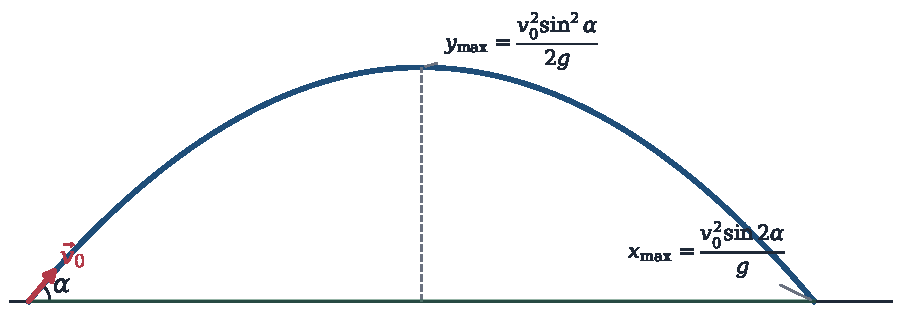
\includegraphics[width=0.78\textwidth]{figures/06_projectile.pdf}
\caption{Parabolic projectile trajectory launched with speed $v_0$ at angle $\alpha$. Velocity vectors $\vec{v}(t)$ remain tangent to the curve, while acceleration $\vec{a} = -g\jhat$ is constant throughout.}
\label{fig:projectile}
\end{figure}

A projectile launched from origin $(0,0)$ with initial speed $v_0$ at launch angle $\alpha$ subject only to uniform gravity $\vec{g} = -g\jhat$ satisfies:
\[
\ddot{x}(t) = 0, \qquad \ddot{y}(t) = -g.
\]
Integrating with initial velocity $\vec{v}_0 = v_0\cos\alpha\,\ihat + v_0\sin\alpha\,\jhat$:
\begin{align*}
v_x(t) &= v_0\cos\alpha = \text{const}, \qquad & x(t) &= v_0\cos\alpha\,t, \\
v_y(t) &= v_0\sin\alpha - gt, \qquad & y(t) &= v_0\sin\alpha\,t - \frac{1}{2}gt^2.
\end{align*}
Eliminating $t = \frac{x}{v_0\cos\alpha}$ yields the \textbf{Cartesian trajectory}:
\[
\boxed{y(x) = x\tan\alpha - \frac{g}{2v_0^2\cos^2\alpha}x^2.}
\]
Since $1/\cos^2\alpha = 1 + \tan^2\alpha$, this can be written as:
\[
\boxed{y(x) = x\tan\alpha - \frac{g x^2}{2v_0^2}\left(1 + \tan^2\alpha\right).}
\]
This is a parabola opening downwards with vertex at:
\[
x_H = \frac{v_0^2\sin(2\alpha)}{2g}, \qquad H_{\max} = \frac{v_0^2\sin^2\alpha}{2g}.
\]
The horizontal range $R$ on level ground ($y = 0, x \ne 0$) is:
\[
\boxed{R = \frac{v_0^2\sin(2\alpha)}{g}.}
\]
\begin{itemize}[leftmargin=1.4em,itemsep=2pt]
  \item Maximum range occurs at $\alpha = 45^\circ$, where $R_{\max} = \frac{v_0^2}{g}$.
  \item Complementary launch angles $\alpha$ and $90^\circ - \alpha$ yield identical horizontal ranges, since $\sin(2(90^\circ - \alpha)) = \sin(180^\circ - 2\alpha) = \sin(2\alpha)$.
\end{itemize}

\section{Circular Motion and Kinematics of Rotation}

\begin{figure}[htbp]
\centering
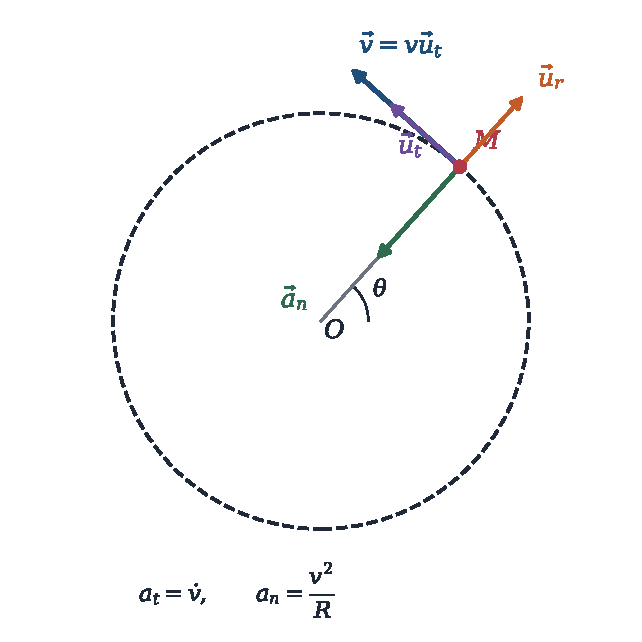
\includegraphics[width=0.74\textwidth]{figures/07_circular_motion.pdf}
\caption{Uniform circular motion of radius $R$. The velocity is strictly tangential $\vec{v} = v\ut$, while the acceleration is purely centripetal $\vec{a} = -\frac{v^2}{R}\ur = -\omega^2 R\ur$.}
\label{fig:circular_motion}
\end{figure}

For a particle moving on a circle of radius $R$, its position is specified by angular coordinate $\theta(t)$:
\[
\vec{r}(t) = R\cos\theta(t)\,\ihat + R\sin\theta(t)\,\jhat.
\]
Differentiating with respect to time:
\[
\vec{v}(t) = R\dot{\theta}\left( -\sin\theta\,\ihat + \cos\theta\,\jhat \right) = R\omega\,\ut,
\]
where $\omega = \dot{\theta} = \frac{\dd\theta}{\dd t}$ is the \textbf{angular velocity} (in $\mathrm{rad\,s^{-1}}$), and linear speed is $v = R\omega$.

Differentiating once more yields the acceleration:
\[
\vec{a}(t) = \frac{\dd}{\dd t}(R\omega\ut) = R\dot{\omega}\,\ut + R\omega\frac{\dd\ut}{\dd t} = R\alpha\,\ut + R\omega(-\omega\ur),
\]
where $\alpha = \dot{\omega} = \ddot{\theta}$ is the \textbf{angular acceleration}.
Thus, the acceleration cleanly splits into two perpendicular components:
\[
\boxed{\vec{a} = \vec{a}_t + \vec{a}_n = R\alpha\,\ut - \omega^2 R\,\ur = R\ddot{\theta}\,\ut - \frac{v^2}{R}\ur.}
\]
\begin{itemize}[leftmargin=1.4em,itemsep=2pt]
  \item The \textbf{tangential acceleration} $a_t = R\alpha = \frac{\dd v}{\dd t}$ changes the \emph{speed} (rate of motion).
  \item The \textbf{centripetal (normal) acceleration} $a_n = \frac{v^2}{R} = \omega^2 R$ points toward the center of curvature and changes the \emph{direction} of the velocity vector.
\end{itemize}

\section{Extensive Worked Examples}

\begin{workedexample}{The Parabola of Safety (Envelope of All Trajectories)}
A coastal defense battery fires shells at a fixed muzzle speed $v_0$, but can vary the launch angle $\alpha \in [0, \pi/2]$ arbitrarily in the vertical plane.
Find the boundary curve in the $(x, y)$ plane that separates points that can be hit by shells from points that are safe from bombardment.

\paragraph{Solution.}

A target at coordinates $(x, y)$ can be hit if and only if there exists at least one real physical launch angle $\alpha$ whose trajectory passes through $(x, y)$.
Recall the trajectory equation expressed in terms of $T \equiv \tan\alpha$:
\[
y = x T - \frac{gx^2}{2v_0^2}(1 + T^2).
\]
Multiply by $\frac{2v_0^2}{gx^2}$ and rearrange into standard quadratic form for $T$:
\[
\frac{gx^2}{2v_0^2}T^2 - x T + \left(y + \frac{gx^2}{2v_0^2}\right) = 0.
\]
This is a quadratic equation $A T^2 + B T + C = 0$ in the unknown $T = \tan\alpha$, with coefficients:
\[
A = \frac{gx^2}{2v_0^2}, \qquad B = -x, \qquad C = y + \frac{gx^2}{2v_0^2}.
\]
Real physical solutions for launch angle $\alpha$ exist if and only if the discriminant $\Delta$ is non-negative:
\[
\Delta = B^2 - 4AC \ge 0.
\]
Evaluating the discriminant:
\[
\Delta = (-x)^2 - 4\left(\frac{gx^2}{2v_0^2}\right)\left(y + \frac{gx^2}{2v_0^2}\right) = x^2 - \frac{2gx^2}{v_0^2}y - \left(\frac{gx^2}{v_0^2}\right)^2 \ge 0.
\]
Dividing by $x^2 > 0$:
\[
1 - \frac{2gy}{v_0^2} - \frac{g^2 x^2}{v_0^4} \ge 0 \implies \frac{2gy}{v_0^2} \le 1 - \frac{g^2 x^2}{v_0^4}.
\]
Multiplying by $\frac{v_0^2}{2g}$:
\[
\boxed{y \le \frac{v_0^2}{2g} - \frac{g}{2v_0^2}x^2.}
\]
The boundary separating hit points ($\Delta > 0$, where two distinct trajectory angles exist: low trajectory and high lob trajectory) from unreachable points ($\Delta < 0$) is the \textbf{Parabola of Safety}:
\[
\boxed{y_{\text{safety}}(x) = H_0 - \frac{x^2}{4H_0}, \quad \text{where } H_0 = \frac{v_0^2}{2g}.}
\]
Every point outside this bounding paraboloid of revolution is completely immune to bombardment.
\end{workedexample}

\begin{workedexample}{Projectile Range on an Inclined Plane}
A projectile is fired with speed $v_0$ at angle $\alpha$ above the horizontal onto a hillside that slopes upward at a constant angle $\beta < \alpha$.
(a) Find the flight time $t_f$ until the projectile strikes the hill.
(b) Calculate the distance $d(\alpha)$ measured along the slope of the hill.
(c) Find the optimal launch angle $\alpha_{\text{opt}}$ that maximizes $d$, and find the maximum range along the incline.

\paragraph{Solution.}

(a) Align a tilted coordinate frame with the $x'$-axis pointing up the incline (angle $\beta$) and $y'$-axis normal to the incline.
In this tilted frame:
\begin{itemize}[leftmargin=1.4em,itemsep=2pt]
  \item Gravity components: $g_{x'} = -g\sin\beta$, $g_{y'} = -g\cos\beta$.
  \item Launch angle relative to incline: $\theta_0 = \alpha - \beta$.
  \item Initial velocity: $v_{x'0} = v_0\cos(\alpha - \beta)$, $v_{y'0} = v_0\sin(\alpha - \beta)$.
\end{itemize}
The motion perpendicular to the incline is:
\[
y'(t) = v_0\sin(\alpha - \beta)t - \frac{1}{2}g\cos\beta\,t^2.
\]
Impact occurs when $y'(t_f) = 0$ ($t_f \ne 0$):
\[
\boxed{t_f = \frac{2v_0\sin(\alpha - \beta)}{g\cos\beta}.}
\]

(b) The distance along the incline is $d = x'(t_f)$:
\[
x'(t) = v_0\cos(\alpha - \beta)t - \frac{1}{2}g\sin\beta\,t^2.
\]
Substituting $t_f$:
\begin{align*}
d &= v_0\cos(\alpha - \beta)\left(\frac{2v_0\sin(\alpha - \beta)}{g\cos\beta}\right) - \frac{1}{2}g\sin\beta\left(\frac{2v_0\sin(\alpha - \beta)}{g\cos\beta}\right)^2 \\
&= \frac{2v_0^2\sin(\alpha - \beta)}{g\cos^2\beta}\left[ \cos(\alpha - \beta)\cos\beta - \sin(\alpha - \beta)\sin\beta \right].
\end{align*}
Using the angle addition identity $\cos(A+B) = \cos A\cos B - \sin A\sin B$ with $A = \alpha - \beta$ and $B = \beta$:
\[
\cos(\alpha - \beta)\cos\beta - \sin(\alpha - \beta)\sin\beta = \cos((\alpha - \beta) + \beta) = \cos\alpha.
\]
Thus:
\[
\boxed{d(\alpha) = \frac{2v_0^2}{g\cos^2\beta}\sin(\alpha - \beta)\cos\alpha.}
\]
Using product-to-sum: $2\sin A\cos B = \sin(A+B) + \sin(A-B)$:
\[
2\sin(\alpha - \beta)\cos\alpha = \sin(2\alpha - \beta) - \sin\beta.
\]
Therefore:
\[
\boxed{d(\alpha) = \frac{v_0^2}{g\cos^2\beta}\left[ \sin(2\alpha - \beta) - \sin\beta \right].}
\]

(c) Since $\beta$ is fixed, $d(\alpha)$ is maximized when $\sin(2\alpha - \beta) = 1$:
\[
2\alpha_{\text{opt}} - \beta = 90^\circ \implies \boxed{\alpha_{\text{opt}} = 45^\circ + \frac{\beta}{2}.}
\]
The optimal launch angle bisects the angle between the incline and the vertical!
The maximum range along the incline is:
\[
d_{\max} = \frac{v_0^2}{g\cos^2\beta}(1 - \sin\beta) = \frac{v_0^2(1 - \sin\beta)}{g(1 - \sin^2\beta)} = \frac{v_0^2(1 - \sin\beta)}{g(1 - \sin\beta)(1 + \sin\beta)} = \boxed{\frac{v_0^2}{g(1 + \sin\beta)}.}
\]
For flat ground ($\beta = 0$), this recovers $\alpha_{\text{opt}} = 45^\circ$ and $d_{\max} = v_0^2/g$.
\end{workedexample}

\begin{workedexample}{The Velocity Hodograph of Projectile Motion}
The \textbf{hodograph} of a motion is the trajectory traced by the tip of the velocity vector $\vec{v}(t)$ in velocity space with coordinates $(v_x, v_y)$.
(a) For a projectile in gravity $\vec{g} = -g\jhat$, sketch the hodograph.
(b) Show that the hodograph is a vertical straight line traversed at constant speed.
(c) Deduce that for any motion with constant acceleration $\vec{a}_0$, the hodograph is a straight line along $\vec{a}_0$.

\paragraph{Solution.}

(a) The velocity vector of a projectile is:
\[
v_x(t) = v_0\cos\alpha = \text{const}, \qquad v_y(t) = v_0\sin\alpha - gt.
\]
In the velocity plane $(v_x, v_y)$, the $v_x$ coordinate never changes ($v_x \equiv v_{x0}$), while the $v_y$ coordinate decreases linearly with time.
Thus, the hodograph is a \textbf{vertical straight line} at distance $v_x = v_0\cos\alpha$ from the $v_y$-axis.

(b) The position vector in velocity space is $\vec{v}(t)$. Its velocity of transit along the hodograph is:
\[
\vec{w}_{\text{hodograph}} = \frac{\dd\vec{v}}{\dd t} = \vec{a}(t) = -g\jhat.
\]
The speed of travel along the hodograph line is constant and equals the gravitational acceleration:
\[
\norm{\vec{w}} = g = 9.81\ \mathrm{m\,s^{-2}} = \text{constant.}
\]

(c) In general, for any particle under constant acceleration $\vec{a}_0$:
\[
\vec{v}(t) = \vec{v}_0 + \vec{a}_0 t.
\]
This is the parametric vector equation of a straight line in velocity space passing through $\vec{v}_0$ parallel to $\vec{a}_0$, traversed with uniform speed $\norm{\vec{a}_0}$. Sir William Rowan Hamilton originally used the hodograph to discover that the velocity locus of planetary orbits is an exact circle!
\end{workedexample}
